\documentclass[11pt]{article}
\usepackage{amssymb}
\usepackage{amsmath}
\usepackage{pst-all}
\usepackage{newicktree}
\usepackage{graphicx}

\title{A Theoretical Foundation for the Age-Area Hypothesis}
\author{\textbf{Matthew J. Baker} \\ Department of Economics \\ Hunter College and the Graduate Center, CUNY}

\begin{document}
\maketitle
\begin{abstract}
\noindent The Age-Area Hypothesis originally advanced by Sapir (1915) is a tool sometimes used to locate the geographical area within which a linguistic stock originated. One common way of stating the hypothesis
is that the area of origin of a linguistic stock is where the languages comprising the stock are maximally differentiated. While the hypothesis is compelling, and its predictions are often corroborated by other evidence, a cohesive theoretical structure for the Age-Area Hypothesis has never been described. This paper describes such a theoretical foundation in terms of probability, and also presents a computational algorithm for computing the relative likelihood that a linguistic stock originated in a given place.
\end{abstract}
\newpage

The age-area hypothesis - evidently first developed by Sapir (1916) in his study of certain Native American Languages - is often invoked, and often implicitly, when linguistic
evidence is summoned in support of the original location of language stocks. Briefly stated, the hypothesis indicates that the geographic area where a language phylogeny originated
is most likely the place where the languages are maximally differentiated.

Examples of the application of this idea abound. Sapir himself used these arguments to suggest that the so-called Na-Dene linguistic grouping originated in and around the North West Coast. As another example, Atkinson and Gray (2003) have used the results to suggest that the Indo-European languages originated in Anatolia, not, as is sometimes supposed, on the steppes of Siberia. Further applications of the idea - either implicit or explicit use of the idea - are almost too numerous to mention.

Another thing that might be said is relative to routes of migration of populations. Such accounts contain many statements to the effect that ``it is probable that'' or ``it is likely'' that population $A$ then bifurcated, and migrated to location $B$, from which point...

What is the existing theoretical basis for the age-area hypothesis? Well, the sister hypothesis in Anthropology - not quite the same idea. In population genetics, it is well known that
the point of maximal genetic diversity of populations is closest their origin. This is because migrants only take a subset of their genes, and cannot have any bearing on the situation
in linguistics.

\section{Problem Description and Motivation}

To be a bit more clear, consider the hypothetical phylogenetic tree displayed in figure \ref{fig1}. This figure shows a language tree comprised
of five languages. A is the most divergent of the group, with B, C, D, E all being more closely related, and D and E being the two most closely
related languages. To avoid forming impressions based on evidence that is not part of the hypothesis, we will suppose that the locations of the
groups have been concealed from us, and that we have no access to archaeological or historical information about the language stock.

In terms of the Age-Area hypothesis and the ultimate source of the tree (i.e., the point at which the tree originated) - one would posit that the point of origin was A's location, as A is the most divergent language from the group. If one wanted to push the hypothesis a bit further, or even apply it recursively, one would come up with a hypothetical migratory route: the hypothesis would lead one to believe that the point of origin of the stock was A, at which point there was a migration from A to B, then from B to C, and then from C to either D or E.

\begin{figure}
\begin{center}
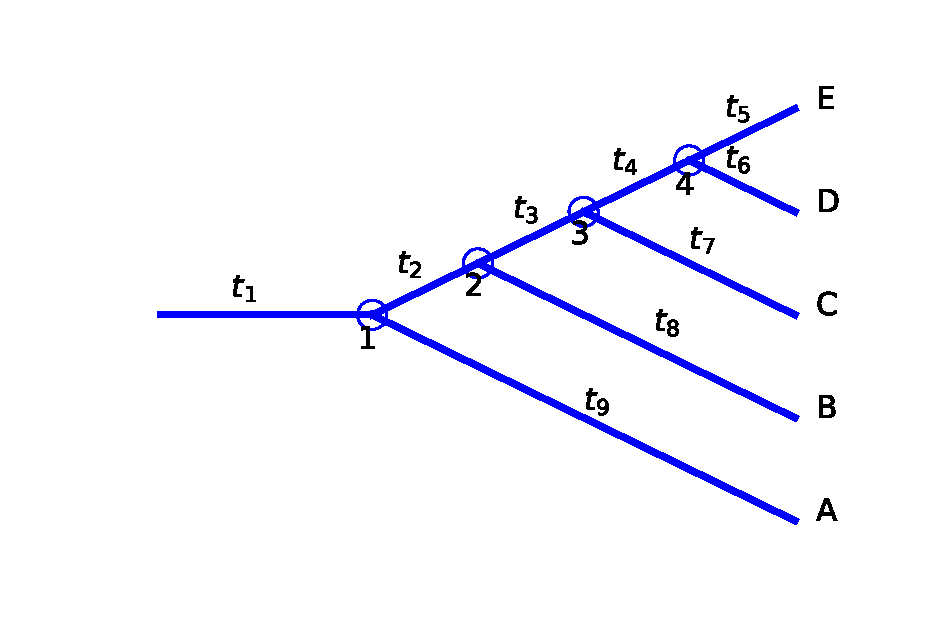
\includegraphics[width=\textwidth]{simplePT.eps}
\caption{A simple phylogenetic tree}
\end{center} \label{fig1}
\end{figure}

There are a large number of other possibilities as well, even though the structure of the tree constrains some sorts of events. For example, an additional plausible sequence of migratory events would be for an initial migratory episode from C to A, followed by another from C to B, followed by yet another migration from C to D or E. These two migratory routes are presented in figure \ref{fig2}.

\begin{figure}
\begin{center}
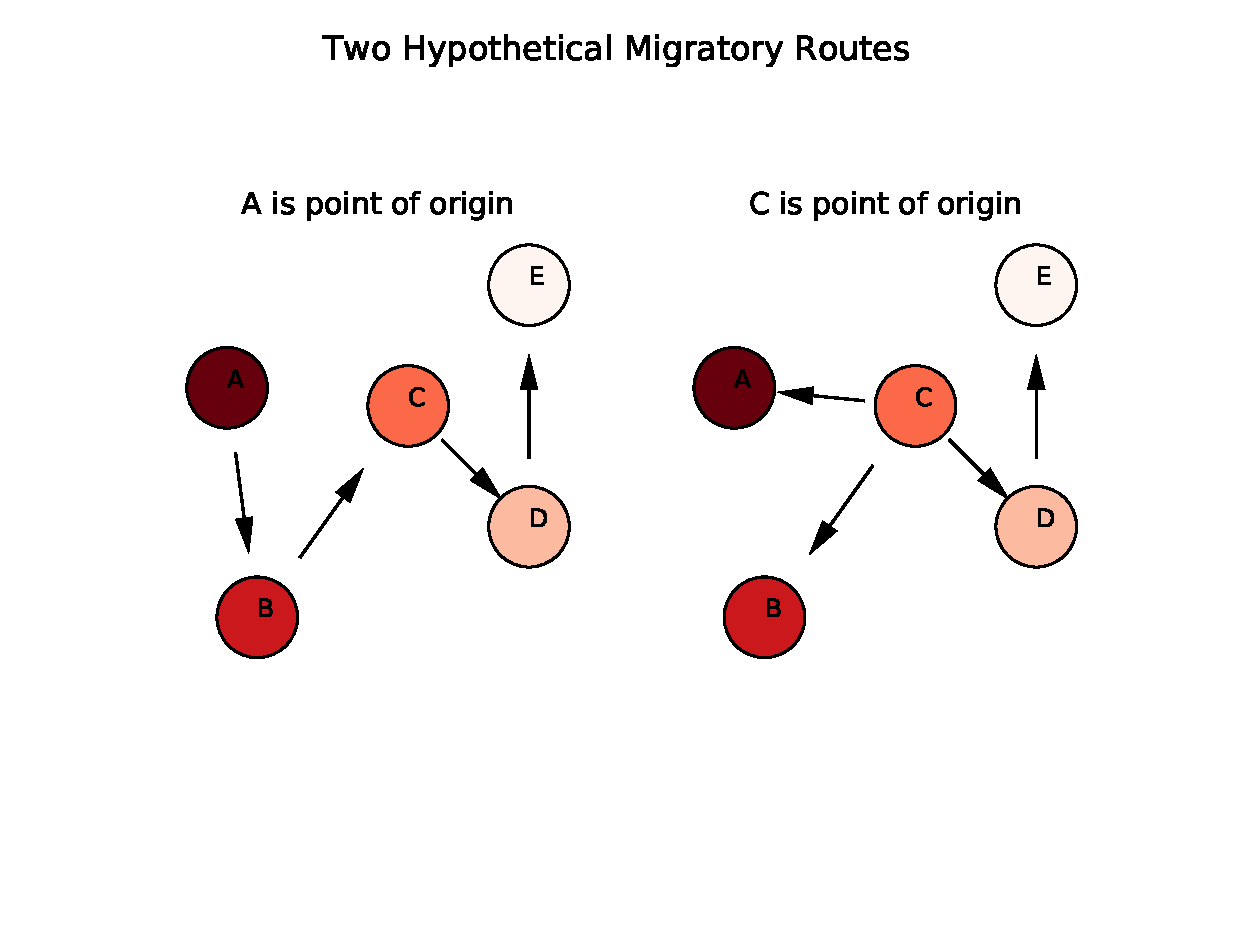
\includegraphics[width=\textwidth]{simpleMR.eps}
\caption{Potential migratory routes among a language stock consisting of five groups, following the Phylogenetic Tree in figure \ref{fig1}}
\end{center} \label{fig2}
\end{figure}

The age area hypothesis suggests that the second sequence of events is somehow less likely than the sequence of events described by the first. Why would one, intuitively, take that to be the case? For a variety of reasons - one might simply appeal to Occam's razor - the events on the left-hand side of figure \ref{fig2} require only one migratory chain, while the events on the right-hand side require three separate expansions: an initial migration from A to C, followed by another from A to B. A third migratory event begins from C continues to D, and then to E. We can now pose our question as follows: if we believe these migratory events to be rare, and we wish to conserve them in explaining historical migrations, what sort of model would accomplish this?

\section{A simple model}

In addition to providing a foundation for the age-area hypothesis, we might lean on some additional principles that we wish to encapsulate in the theory. We might like the model to conserve on estimation of parameters, and we might also like the model to have a consistent internal logic. A simple model with transparent machinery also creates the possibility of expansion and further development. While the assumptions listed below are restrictive, one can see how they might be relaxed in future work.

Accordingly, let's make the following assumptions:
\begin{enumerate}
\item The entire phylogenetic tree is observed; there are no unobserved migratory events.
\item A group arrives in its current position with we might call a ``propensity to migrate.'' It then discharges an additional migratory rate with exponential density.
\item Once a group arrives in its current and discharges a migratory group, it is then dormant; subsequent migration from the group's location requires the beginnings of an additional migratory episode.
\end{enumerate}

One good thing about this model is that it can be easily concentrated. That is, the parameters of any exponential distribution can be concentrated out of the likelihood, and this makes the workings of the model clear in that one can easily see how and why it would posit that the first sequence of events on figure \ref{fig2} are more likely.

To see the basic idea, let's develop a comparison of the two scenarios described in figure \ref{fig2}. The first scenario requires an initial migratory event to start after time $t_0$ from point $A$. At this point, according to the model assumptions, $A$ is dormant, and the migratory bug is transitioned to location $B$. After time $t_1$, $B$ emits the migratory bug to $C$ and is then dormant, followed by $C$'s emission and subsequent dormancy, and then $D$'s. Finally, $E$ retains the bug but never emits. 

This is the only migratory episode needed to explain the positioning of the groups in the tree, and given the assumption that discharges are exponential, suppose our events are described by the distribution $\textrm{Exp}(\lambda)$. Then, we have the likelihood of point $A$ being the point of origin as:
\begin{equation} \label{e1}
P_A = \lambda e^{-\lambda t_0}\lambda e^{-\lambda t_1}\lambda e^{-\lambda t_2}\lambda e^{-\lambda t_3}e^{-\lambda t_8}
\end{equation}
or 
\begin{equation} \label{e2}
P_A = \lambda^4 e^{-\lambda (t_0+t_1+t_2+t_3+t_8)}
\end{equation}

There are a couple of points of interest for equation (\ref{e1}). First, since only one migratory path is needed to explain the events, only one
exponential parameter is needed for the whole process. Also, since a migratory event after $t_8$ is never observed, we have $1-F(t_8,\lambda) = e^{-\lambda t_8}$; there is only one such ``operational branch'' when our observation period ends. 

Since the migration parameter is not of as great of interest as the probability, we can take the log of equation $\ref{e2}$ and maximize the result with respect to $\lambda$, and substitute the result back in to concentrated likelihood, giving us a closed-form expression for the probability that $A$ is the point of origin:
\begin{equation} \label{e2}
P_A = \frac{4^4e^{-4}}{(t_0+t_1+t_2+t_3+t_8)^4}
\end{equation}
Of course, this is not all that meaningful without a point of comparison. So, by way of comparison, according to this model, what is the likelihood that the point of origin is $C$? 

In this case, the process begins with a migration after $t_0$ from $C$ to $A$. Subsequently, no additional migrations occur from $A$, so $A$ remains active. Then, after time $t_1$ a second migratory event arises leading from $C$ to $B$, after which nothing further occurs on this branch. Then, a migratory event leads from $C$ to $D$ over time $t_2$, and then from $D$ to $E$ over time $t_3$, at which point nothing more happens. 

The key thing about this explanation is that there are three separate migratory events needed to explain things, so we need three exponential parameters in the model. Another key thing is that we have more branches that are ``alive'' at the end of the process. These might suggest intuitively that this explanation is less likely than the previous, and this is indeed the case under the model. Forming the likelihood in the
same way as we did above, we have:
\begin{equation} \label{e3}
P_C = \lambda_1e^{-\lambda_1(t_0+t_4)} \lambda_2 e^{-\lambda_2 (t_1+t_5)}\lambda_3^2 e^{-\lambda_3 (t_2+t_3+t_8)}
\end{equation}
So, here we have a three-parameter model, which is how the increased complexity of the explanation (the anti-Occam's razor effect) is manifest in the probability. Concentrating \ref{e3} as above gives the result:
\begin{equation} \label{e4}
\frac{2^2e^{-4}}{(t_0+t_4)(t_1+t_5)(t_2+t_3+t_5)}
\end{equation}

 We can form the ratio of this and the previous expression and see which tree is more likely under which configuration of the parameters. The intuition behind the explanation can be written as: 
 \begin{equation*}
 LR = 4\left({1-\frac{t_0}{T}}\right)4^2\left(1-\frac{t_o+t_1}{T}\right)^2
 \end{equation*}
So we see that unless the branches $t_0$ and $t_1$ constitute a (very) large span of the tree, our model claims that $A$ is the most likely place of origin. 

\section{An algorithm}

As is often the case when dealing with estimation over trees, it behooves one to consider an algorithm that works backwards from the branches to the base. The algorithm presented here is essentially a pruning algorithm like Felsenstein's with a hint of dynamic programming. The dynamic programming aspect introduces a sort of continuation maximum likelihood into the tree. 

The algorithm works as follows. At termination, the result is a concentrated log-likelihood of each location being the point of origin.  The following is an illustration showing how the algorithm works on the example given above. 

\begin{enumerate}
\item[0.] Initialization: a ``active'' vector of zeros $A=[0,0,0,0,0]$, a vector of exponential parameters that start with zero, $E=[0,0,0,0,0]$, and a continuation likelihood $L=[-t_4,-t_5,-t_6,-t_7,-t_8]$
\item  Select an interior node and pick out its branches. 
\item  Poo
\end{enumerate}








\end{document} 